\ylDisplay{Keha vees} % Ülesande nimi
{Koit Timpmann} % Autor
{lõppvoor} % Voor
{2019} % Aasta
{P 6} % Ülesande nr.
{3} % Raskustase
{
% Teema: Mehaanika
\ifStatement
Õpetaja näitas tunnis katset. Kangkaalu ühes kaalukausis oli klaas veega, teises kaalukausis statiiv, mille varda küljes rippus alumiiniumist keha. Kaal oli tasakaalus. Nüüd lasi õpetaja statiivivarda koos selle otsas rippuva kehaga alla, nii et keha sukeldus üleni klaasis olevasse vette. Kui suure massiga lisakoormis tuleb ühele kaalukausile asetada, et kaal oleks uuesti tasakaalus? Kummale? Rippuva keha mass $m = 135$ g. Alumiiniumi tihedus $\rho Al = 2700$ $kg/m^3$ , vee tihedus $\rho_v = 1000$ $kg/m^3$.
\begin{center}
	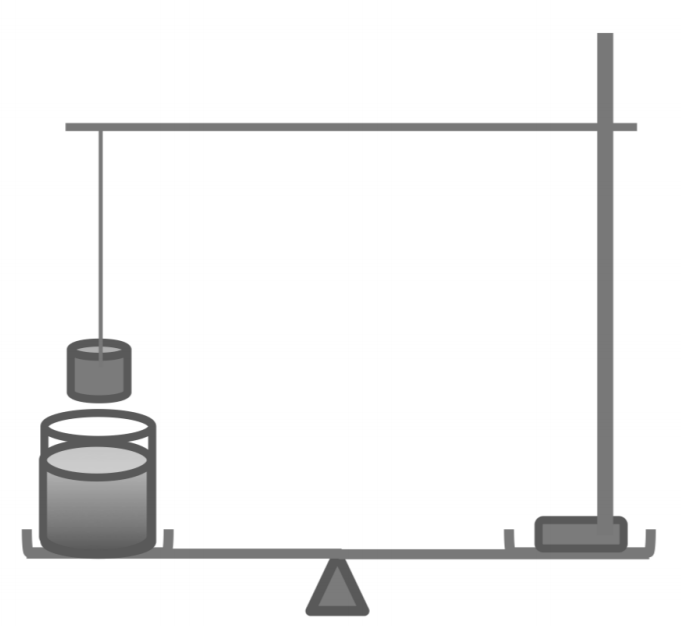
\includegraphics[width=0.5\linewidth]{2019-v3p-06-yl.PNG}
\end{center}
\fi

\ifHint
Pärast keha vettelaskmist mõjuvad parempoolsele kaalukausile järgmised jõud: statiivile mõjuv raskusjõud + kehale mõjuv raskusjõud – kehale mõjuv üleslükkejõud. Vasakule kaalukausile mõjub klaasile, veele ja keha poolt väljatõrjutud veele mõjuv raskusjõud.
\fi

\ifSolution
Vette lastud koormisele mõjub üleslükkejõud
\begin{center}
$F = \rho_v gV_k$.
\end{center}
Keha ruumala saame tiheduse valemist
\begin{center}
$\rho = m/V$, millest $V = \frac{m}{\rho}$.
\end{center}
Üleslükkejõud mõjub vettelastud kehale üles. Seega pärast keha vettelaskmist mõjuvad parempoolsele kaalukausile järgmised jõud: statiivile mõjuv raskusjõud + kehale mõjuv raskusjõud – kehale mõjuv üleslükkejõud. Seega mõju parempoolsele kaalukausile väheneb kehale mõjuva üleslükkejõu võrra. Vettelastud keha tõttu vedeliku tase klaasis tõuseb ning vedeliku rõhk anuma põhjale suureneb. Seega mõjub vasakule kaalukausile klaasile, veele ja keha poolt väljatõrjutud veele mõjuv raskusjõud. Pärast keha vette laskmist väheneb üleslükkejõu võrra paremale kaalukausile mõjuv jõud ja suureneb üleslükkejõu võrra vasakule kaalukausile mõjuv nõud. Et kaal tasakaalustada, tuleb statiiviga kaalukaussi lisada koormis, mille massile mõjub kahekordne üleslükkejõud.
\begin{center}
$F = \frac{2 \cdot 1000 km/m^3 \cdot 9,8 N/kg \cdot 0,135kg}{2700 kg/m^3} = 1$ N
\end{center}
Kuna
\begin{center}
$F = mg$, siis $m = \frac{F}{g} = \frac{1 N}{9,8 N/kg} = 0,1$ kg
\end{center}
\fi
}